\section*{Supplementary Information}
\setcounter{figure}{0}
\renewcommand{\thefigure}{S.\arabic{figure}}
\setcounter{table}{0}
\renewcommand{\thetable}{S.\arabic{table}}
\setcounter{subsection}{0}
\renewcommand{\thesubsection}{S.\arabic{subsection}}
\setcounter{equation}{0}
\renewcommand{\theequation}{S.\arabic{equation}}

\subsection{Memory lifetime \label{lifetime}}
There are three effects limiting the lifetime of this ORCA memory: spontaneous emission from the doubly excited atomic state, motion-induced dephasing due to the Doppler effect, and destructive interference between hyperfine components of the excited state.

Motion-induced dephasing arises due to the Doppler effect and atomic motion in a warm ensemble. This is because the stored excitation is spread over atoms belonging to different velocity classes in the ensemble. Due to the Doppler effect, each velocity class experiences the signal and control fields shifted in frequency. As a consequence, the phase of the stored coherence evolves at different rates in different velocity classes. The motion-induced dephasing lifetime is \cite{Zhao2009} $\tau_D = k_r v_s$, where $v_s = \sqrt{k_B T/m}$, and $k_r=\frac{2\pi}{\lambda_\mathrm{s}} -\frac{2\pi}{\lambda_\mathrm{c}}$; with $T$ the temperature of the atomic vapour, $m$ the mass of the atom, and $\lambda_\mathrm{s/c}$ the wavelengths of the signal and control fields. In other words, the collective coherence will dephase at a rate proportional to the square root of the temperature, and the wavenumber mismatch of the fields.

In the absence of optical pumping, the off-resonant two-photon excitation that stores the signal photon has contributions from all allowed paths connecting the $6S_{1/2}$ and $6D_{5/2}$ manifolds. The resulting excitation is spread across components of the $6D_{5/2}$ manifold. During storage time these components oscillate with different rates as given by their energy differences, and at read-out time they can interfere destructively in the creation of the read-out photon. Optical pumping restricting the memory interaction to the hyperfine levels $F=4 \rightarrow F=5 \rightarrow F=6$ reduces this effect.

\begin{figure}[h]
\centering
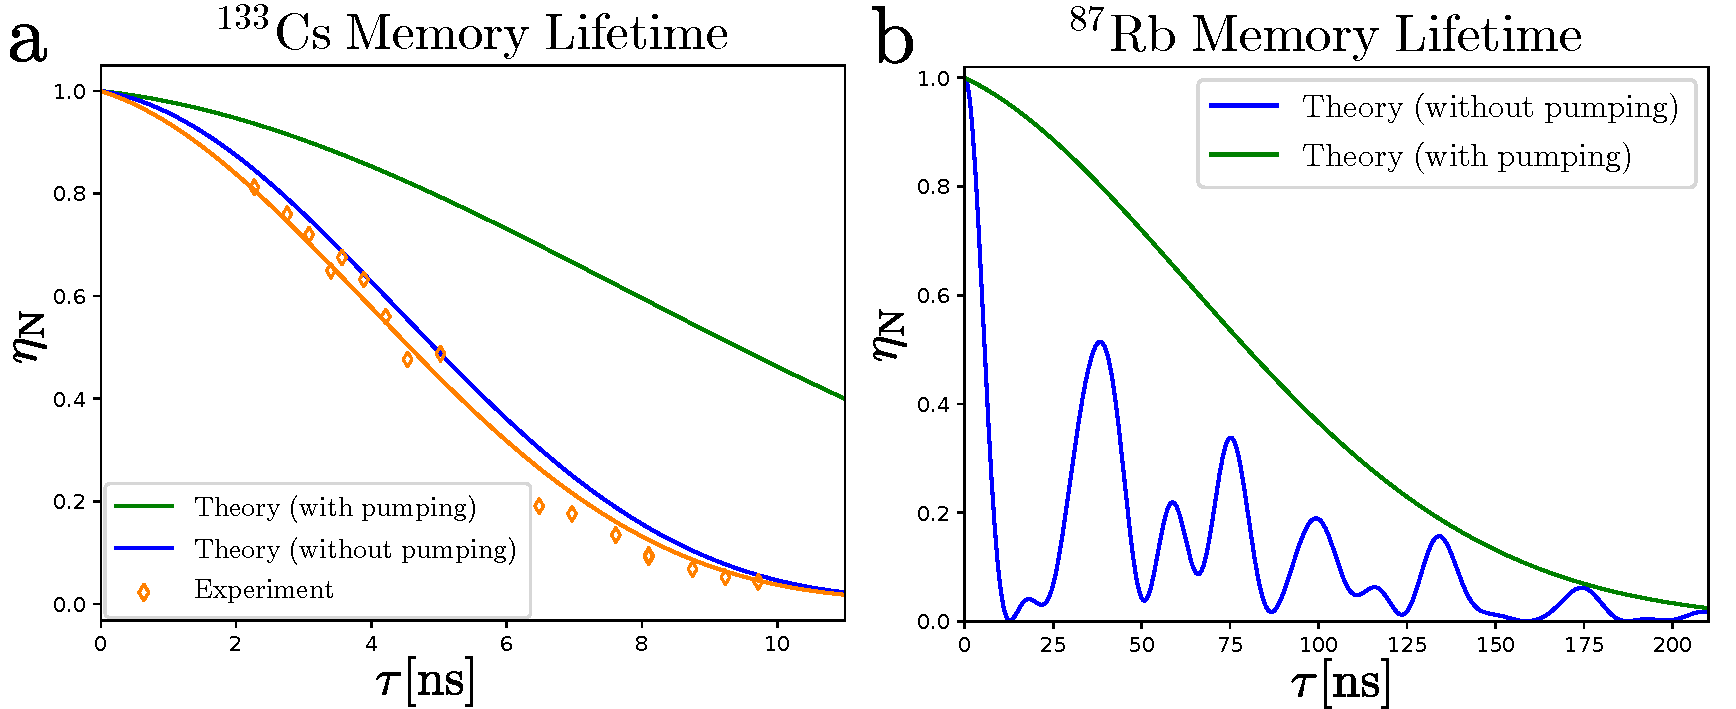
\includegraphics[width=\linewidth]{lifetime_cs_rb.pdf}
\caption{\textbf{a}. The measured (normalised to $\tau=0$) memory efficiency $\eta_\mathrm{N}$ (orange diamonds, experimental errors are smaller than the markers) versus storage time $\tau$ along with a theory fit of the memory lifetime curve (orange line) yielding a (1/e) lifetime of $5.5\pm0.1$ ns. Also shown is the predicted memory lifetime curves with (green) and without (blue line) optical pumping. \textbf{b}. Memory lifetimes predicted from theory for $^{87}\mathrm{Rb}$ with (green) and without (blue line) optical pumping.}
\label{fig:figLifetime}
\end{figure}

We determine the actual memory lifetime by measuring the memory efficiency for different storage times using a weak coherent state signal. In Fig. \ref{fig:figLifetime}a we show the measured normalized memory efficiency versus storage time (orange diamonds). Fitting our model to the data we obtain a $1/e$ lifetime of $5.5\pm 0.1$ ns. Using the Maxwell-Bloch model directly we predict a memory lifetime of 5.9 ns, very close to the measured one.

While seemingly short, the memory lifetime can be extended through optical pumping to reduce the destructive interference of hyperfine components or by using a different atomic species with a smaller signal/control wavenumber mismatch. If we choose the dipole couplings in the model such that only the transition $F=4 \rightarrow F=5 \rightarrow F=6$ is allowed (as with optical pumping), we obtain a memory lifetime of 11.5 ns (the green curve in figure \ref{fig:figLifetime}a). Furthermore, a simulation of the $5S_{1/2}\rightarrow5P_{3/2}\rightarrow5D_{5/2}$ cascade in $^{87}\mathrm{Rb}$ (signal at 780~nm, control at 776~nm) yields a memory lifetime of $99$~ns as shown by the green curve in \ref{fig:figLifetime}b.

\subsection{Experimental setup \label{setup}}

\begin{figure}[h!]
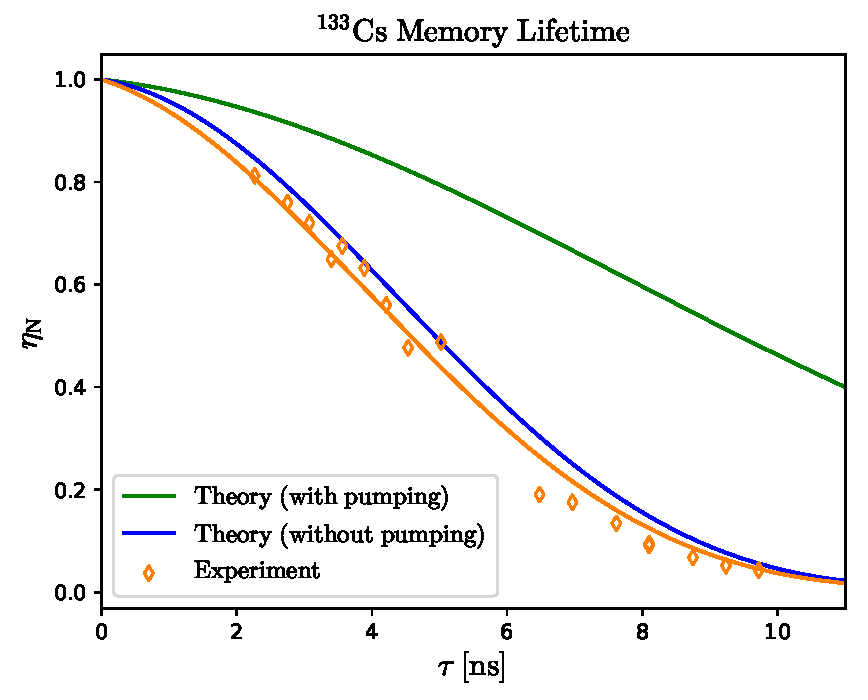
\includegraphics[width=\textwidth]{doppler_dephasing_cs3.pdf} % this command will be ignored
\caption{\textbf{Schematic of the experimental setup for ORCA}. \textbf{(a) }  Signal generation stage. \textbf{(b) } Control generation stage. \textbf{(c) } Memory and detection stage. SHG - periodically poled potassium titanyl (ppKTP) bulk crystal; ppKTPw - ppKTP waveguide; DM - dichroic mirror; FP - Fabry-P\'erot etalon; PBS - polarizing beamsplitter; HWP - half-wave plate; QWP - quarter-wave plate; APD - avalanche photodiode detector; BF - bandpass filter.}\label{fig:figSup1}
\end{figure}

Figure \ref{fig:figSup1} shows a schematic of the ORCA experimental setup. For the memory lifetime measurement (section \ref{lifetime}) we produce a weak coherent state signal (average photon number of $\sim2$) by picking pulses using a fast Pockels cell (extinction ~20,000:1) at a 1 MHz rate from a 80 MHz train of pulses generated by a $\sim330$ ps actively mode-locked titanium sapphire (Ti:Sapph) laser operated at 852 nm and filtered by a Fabry-P\'erot (FP) etalon down to 0.81 GHz bandwidth. Using a scanning FP etalon connected to a PC running LabVIEW, we reference-lock the Ti:Sapph's center frequency (via the voltage on a Gires-Tournois-Interferometer inside the laser cavity) to a continuous wave (CW) laser locked to the Cs D2 line via saturated absorption spectroscopy. 

We generate the control field from a second $\sim500$ ps actively mode-locked Ti:Sapph laser operated at 917 nm, with its center frequency locked using a wavelength meter, and its repetition rate locked to the signal Ti:Sapph using a commercial lock-to-clock (L2C) system. We use an unbalanced free-space Mach-Zehnder interferometer to split the 80 MHz pulse train into two, with a variable delay $<\sim4$ ns between them, in order to investigate storage times $<12.5$ ns. For storage times $6\;\mathrm{ns}<\tau<12.5$ ns we use the L2C electronics to change the timing between signal and control pulse trains such that read-in and read-out are switched. We also use the L2C to temporally overlap the signal and control pulses in the memory cell.

We combine the signal and control fields on a dichroic mirror, which - followed by a 10 nm bandpass filter centred at 850 nm - reduces control field leakage to the detectors from back-reflections by a factor of $\sim10^9$. We focus signal and control beams down to a $\sim300\;\mu$m waist inside a 72 mm -long uncoated caesium borosilicate reference cell heated using a custom-made oven. We estimate the cell temperature to be $\sim 91^o$C by frequency scanning a weak CW probe laser over the Cs D2 line and fitting a Voigt profile to the measured atomic absorption line.

After the signal field passes through the memory and the filters, we send it into a Hanbury-Brown-Twiss setup, composed of a half-waveplate, polarising beamsplitter and two fibre-coupled single-photon avalanche photodiodes. The two signal and the idler avalanche photodiodes were connected to a time-to-digital converter. For the weak coherent state data and cross-correlation measurements, we add the counts on the two signal detectors to estimate the total magnitude of the transmitted/recalled signal.

\subsection{Photon source and setup losses}
The generation of heralded single photons is achieved using type-II parametric down-conversion in a ppKTP waveguide. The waveguide, operated in a single-pass configuration and of length 20$\,$mm, is pumped with pulses of approximately 270 ps duration at a wavelength of 426\,nm. This pump light is derived by doubling the above mentioned 852\,nm Ti:Sapph laser via second harmonic generation in a separate 2$\,$mm long ppKTP crystal. With an incident average power near 700\,mW at 852\,nm at the crystal we arrive with 4\,mW average power at 426\,nm before the PDC waveguide. This light is then coupled to the waveguide with a total transmission of $<10\%$ including the loss at the in- and out-coupling lenses. We note that the waveguide is not single-mode for the pump wavelength and that the coupling is optimised to primarily excite the fundamental spatial mode, resulting in a low overall transmission. The generated frequency-degenerate but polarisation-orthogonal signal and idler modes have a bandwidth on the order of $1\,$THz. 

We characterise beam propagation transmission using an ``alignment'' mode, which is coupled to the fundamental mode of the waveguide, and thereby comparable to the signal and idler modes allowing for ``classical'' measurements to be made. These modes are then subject to frequency filtering. First, we apply coarse filtering using edge filters. Then, the modes are spatially separated via a PBS to then be coupled to their own single-mode fibre (SMF) with an efficiency of $(64 \pm 1)\%$ for the signal mode and $(53 \pm 2)\%$ for the idler mode. The modes are then out-coupled and recombined on a PBS forming a common spatial mode to then pass two etalons, one of FSR$\,$=$\,$18.4$\,$GHz and one of $103\,$GHz, which gives an effective FSR of $~1\,$THz (lowest common multiple). This is followed by a holographic volume Bragg grating with a width $\sim$100$\,$GHz. Using a narrowband ($\sim\,$MHz) probe the measured width this filtering has is $1\,$GHz for both modes. Finally the modes are separated spatially again via a PBS, the idler coupled to an APD (efficiency $\eta \approx 50\%$, dark counts = $163\pm 1\,$Hz) via a multimode fibre (total transmission from after waveguide to in front of idler detector is $\eta_\textrm{i,filt}\,=\,(9.7\pm0.1)\,\%$), while the signal is coupled to a SMF to be out-coupled and steered to the memory (total transmission from after waveguide to after this SMF is $\eta_\textrm{s,filt}\,=\,(12.8 \pm 0.3)\,\%$). 

The filtered signal photon is now steered toward the memory. First there is an edge filter which is used to prevent the 917$\,$nm control from backward-coupling toward the source which presents additional loss to the signal mode. Further, the caesium cell used is uncoated, adding more loss. After passing the cell, the signal mode is then separated from the control mode via a dichroic mirror and finally passes a bandpass filter about 852$\,$nm before entering a Hanbury-Brown-Twiss set-up. The mode is spatially separated into two and coupled to two APDs ($\eta\approx50\,\%$ dark counts = $296 \pm 2\,$Hz and $\eta\approx50\,\%$ dark counts = $356 \pm 2\,$Hz) via SMF. The total transmission from the source to in front of these detectors (averaging over the two SMF couplings) is $\eta_\textrm{s,total}\,=\,3.7\pm0.1\,\%$. That is to say, the photon undergoes an additional $\eta_\textrm{s,add}\,=\,30\,\%$ transmission from after the initial filtering stage.

For all results presented in this paper we operated with an average pump power of $4\,$mW in front of the waveguide in-coupling lens. Typically, we measure an idler (signal) count rate of around $30\,$kHz ($10\,$kHz) for the case of no control pulses. The typical Klyshko efficiency $\eta_k$ measured is $0.7\,\%$. This allows to calculate a heralding efficiency of $\eta_\textrm{herald} = \eta_k/\eta_{\textrm{det}}/\eta_\textrm{s,add} = 4.7\,\%$, which is well above the $\mu_1$ of the memory, as required for single-photon storage \cite{Gundogan2015}. Finally, the heralding efficiency just after the waveguide is $\eta_\textrm{s,waveguide} = \eta_k/\eta_{\textrm{det}}/\eta_\textrm{s,total} = 38\,\%$. The missing factor of $2.6$ we attribute to not measuring explicitly the loss inside the waveguide, the out-coupling loss from waveguide to free-space and the potential frequency mismatch of the etalon centroids between signal and idler.

\subsection{Data acquisition and post-processing}
During the measurements, the settings of three mechanical shutters which selectively blocked the read-in, read-out, and signal beams defined four different configurations (see Fig. \ref{fig:measurement_settings}): memory measurements with all three shutters open ("MEM"); read-in measurements with signal and read-in shutters open, and read-out shutter closed ("RI"); signal measurements with signal shutter open and both read-in and read-out closed ("SIG"); and noise measurements with read-in and read-out shutters open and signal shutter closed ("CTRL"). A single measurement consisted of recording the number of detector counts registered in a period of 180~s in the "MEM" configuration, followed by recording the total counts over 10~s in the "RI", "SIG", and "CTRL" configurations. After completion of all four configurations, the corresponding data was written to disk and the measurement repeated. This mode of operation was chosen in order to mitigate the effect of slow drifts in the setup that arose from changes in the laboratory temperature and humidity.

\begin{figure}[h!]
\centering
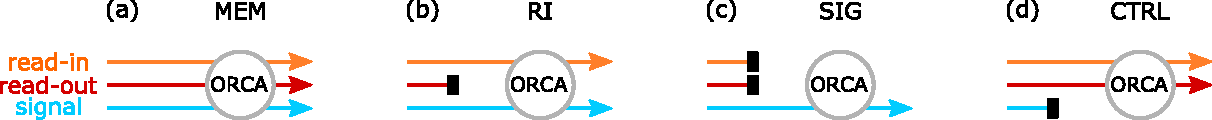
\includegraphics[width=\linewidth]{Sup1KTK.pdf}
\caption{\textbf{Schematic of the different measurement settings.} Black rectangles signify a closed shutter. For more information see the text.}
\label{fig:measurement_settings}
\end{figure}

For each configuration in each measurement, we recorded arrival time histograms for the three detectors ($\mathrm{D_{i}}$, $\mathrm{D_{s1}}$, $\mathrm{D_{s2}}$). These are histograms of firing times of the single-photon detectors with respect to a 1~MHz trigger signal derived from the Ti:Sapph recorded with the time-to-digital converter (TDC). We chose a time-bin width of 200~ps as a compromise between temporal resolution of the TDC and total number of time bins in the histogram. For data visualization, we added all arrival time histograms and normalised them to both the number of measurements (521) and the respective measurement duration (180~s for "MEM", 10~s else), obtaining a count rate per time bin in units of Hertz. 

Fig. \ref{fig:arrival_time_02} shows a section of the arrival time histograms. To reduce the impact of spurious noise counts (primarily from detector dark counts), we applied time gates to the recorded arrival time histograms and only kept events that lay within the time gates. The time gates for the read-in pulses (blue regions) are centred around the maxima of the individual read-in peaks and have a width of 2.5 ns, chosen such that the peaks were completely inside the gating region. Similar time gates were chosen for the recalled light, where the centre of these read-out gates (orange regions) was offset from the corresponding read-in time gates by 3.5 ns, which was the storage time chosen for the experiment. By integrating the detection events over only the gate regions, we calculated the read-in, read-out, and total memory efficiencies stated in the main text.  

\begin{figure}
\centering
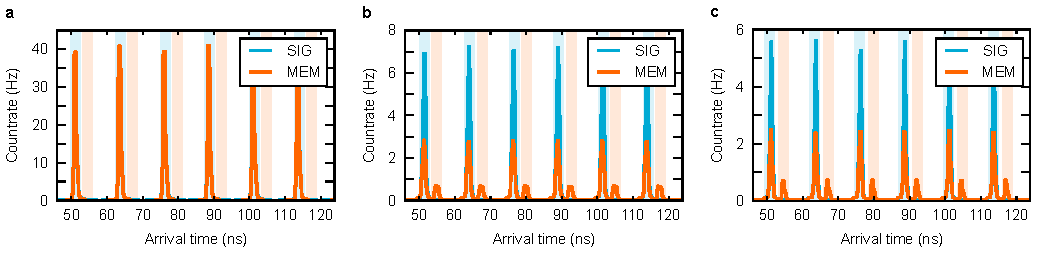
\includegraphics[width=\linewidth]{supplements_arrival_time_02.pdf}
\caption{\textbf{Sections of the arrival time histograms with indicated time gates.} \textbf{a} A section of the arrival time histogram for $\mathrm{D_{i}}$ We show the histograms for the "SIG" (blue trace) and "MEM" (orange trace) configuration. \textbf{b} A section of the arrival time histograms for detector $\mathrm{D_{s1}}$. \textbf{c} The same for detector $\mathrm{D_{s2}}$. For more details see the text.}
\label{fig:arrival_time_02}
\end{figure}

In addition to the arrival time histograms, we also recorded coincidence histograms for signal-idler two-fold coincidences ($\mathrm{D_i}$-$\mathrm{D_{s1}}$, $\mathrm{D_i}$-$\mathrm{D_{s2}}$) and the three-fold coincidences ($\mathrm{D_i}$-$\mathrm{D_{s1}}$-$\mathrm{D_{s2}}$). These are start-stop histograms, where the detection of an idler photon starts the measurement and the detection of a signal photon (the detection of a $\mathrm{D_{s1}}$-$\mathrm{D_{s2}}$ coincidence) serves as the stop signal for the two-fold (three-fold) coincidence measurement. Here, the time-bin width of the TDC was chosen to be 100~ps to ensure that the temporal resolution of the measurement was not limited by the TDC, and the time gates had a width of 3.5 ns. Again, the data was post-processed for visualization similar to the arrival time histograms. The resulting coincidence traces are plotted in Fig. \ref{fig:correlations}. Note that the unconventional shape of the traces originates from the logarithmic scaling of the y axes.

\begin{figure}
\centering
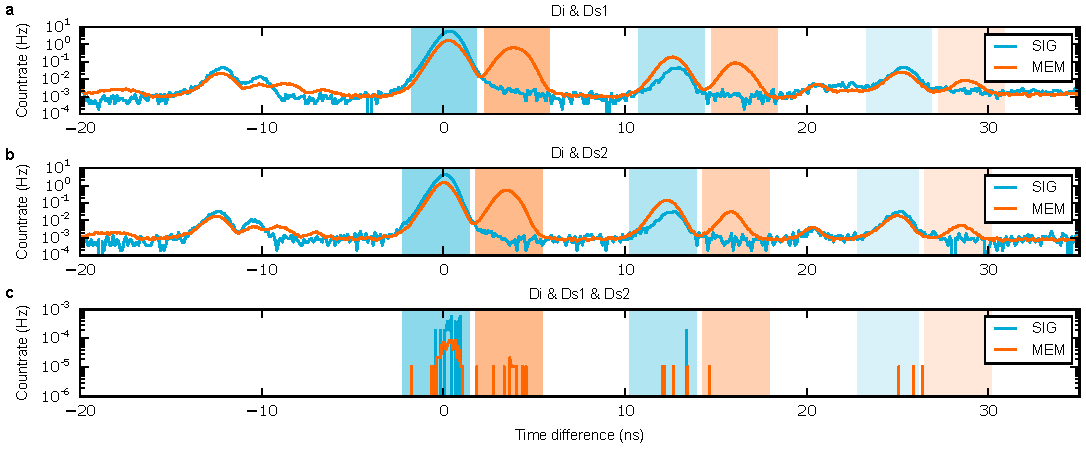
\includegraphics[width=\linewidth]{supplements_correlation.pdf}
\caption{\textbf{Correlation histograms.} \textbf{a} Accumulated normalised correlation histogram for two-fold coincidences between detectors $\mathrm{D_{i}}$ \& $\mathrm{D_{s1}}$, shown for the "SIG" (blue trace) and "MEM" (orange trace) configurations. Note the logarithmic scaling of the y axis. In the main text, we analyse the $g^{(1,1)}(0)$ cross-correlation for the initial time at 0~ns (read-in; blue-shaded) and 3.5~ns (read-out; orange-shaded). Successive read-in (read-out) time bins are indicated by shaded regions with decreasing saturation. \textbf{b} The same as in \textbf{a}, now however for two-fold coincidences between detectors $\mathrm{D_{i}}$ \& $\mathrm{D_{s2}}$. \textbf{c} Correlation histogram for three-fold coincidences between detectors $\mathrm{D_{i}}$ \& $\mathrm{D_{s1}}$ \& $\mathrm{D_{s2}}$.}
\label{fig:correlations}
\end{figure}

The "SIG" traces show a dominant peak at a time difference of 0~ns, with subsequent smaller peaks at integer multiples of the laser repetition time of 12.5~ns. From this we calculate the $g^{(1,1)}$ signal-idler cross-correlation function. The results for the "SIG" configuration are summarized in the first row of Tab. \ref{tab:g11}, where we find $g^{(1,1)}=131(1)$ for a time difference of 0~ns and $g^{(1,1)}\approx1$ for integer multiples of 12.5~ns. We also note that the values at the read-out times (3.5~ns offset from the 12.5~ns time slots) are meaningless, since there is no actual signal at the detectors. 

Turning our attention to the "MEM" configuration (orange traces in Fig. \ref{fig:correlations}), we again find a dominating peak at a time difference of 0~ns with side peaks at integer multiples of 12.5~ns. In addition, we see peaks that are offset from the major peaks by 3.5~ns. These originate from coincidence events between idler photons and signal photons that have been stored in and recalled from the memory. We also note that the side peak at 12.5~ns is higher than the corresponding peak for the "SIG" configuration. The reason for this lies in the non-unity read-out efficiency of our memory. A stored photon is not necessarily read out after 3.5~ns, but can remain stored in the memory. Then, it can be read out by the next laser pulse arriving at 12.5~ns, and so on. To quantify this effect, we again evaluate $g^{(1,1)}$. The results are summarized in the second row of Tab. \ref{tab:g11}. In this case, we find non-classical values for $g^{(1,1)}$ up to a time of 16~ns, which corresponds to around three times the lifetime of our memory. These results highlight the noise-free operation of ORCA: non-classical photon correlations are retained even after the memory efficiency has decayed to around 5\% of its initial maximum value ($1/e^3$).

\begin{table}
\centering
\begin{tabular}{|l||l|l|l|l|l|l|}
\hline
\multirow{2}{*}{}   & \multicolumn{6}{c|}{$g^{(1,1)}$} \\
%\hline
    & $\tau=0$ ns & $\tau=3.5$ ns & $\tau=12.5$ ns & $\tau=16$ ns & $\tau=25$ ns & $\tau=28.5$ ns \\
\hline\hline
SIG & 131(1) & 0.203(1) & 1.13(2) & 0.0773(1) & 1.23(2) & 0.137(1) \\
\hline
MEM & $80.5(1)$ & $120(1)$ & $9.74(2)$ & $11.3(1)$ & $1.78(2)$ & $1.19(1)$ \\
\hline
\end{tabular}
\caption{\textbf{Cross-correlation for successive read-outs.} Calculating $g^{(1,1)}$ for higher-order read-outs at integer multiples of $12.5$ ns (plus 3.5 ns for read-out pulses) yields the preservation of non-classical correlations by the memory up to around three times the memory lifetime.}
\label{tab:g11}
\end{table}